% UONTEST.TEX - a sample file for the UONTHESIS document style.
% revised by Colin Johnson (Colin.Johnson@nottingham.ac.uk), 2020-02-18
%
\documentclass[11pt]{uonthesis}

\usepackage[titletoc]{appendix}
\usepackage{graphicx, multirow, multirow, subcaption, amsmath} % put additional packages here
%\usepackage[backend=biber, sorting=nyt, style=numeric, firstinits=true]{biblatex}
\bibliographystyle{acm} 
%\addbibresource{refs.bib}

\renewcommand{\appendixtocname}{List of appendices}

\title{Real-time prediction of lane-level traffic speeds using Mixed Deep Learning model with Apache Spark and Kafka}
\author{Makoto Ono}
\prevdegrees{MSc}
\university{The University of Nottingham}
\degree{Master of Science in Computer Science with Artificial Intelligence}
\date{September 2024}

%%%%%%%%%%%%%%%%%%%%%%%%%%%%%%%%%%%%%%%%%%%%%%%%%%%%%%%%%%%%%%%%%%%%%%%%%%%%%%%%%%%%
\begin{document}

\begin{frontmatter}
\maketitle
\tableofcontents

\begin{abstract}
According to the guidelines the abstract should not exceed 300 words.
However, it is unlikely that anyone will be counting when you submit.
If you still wish to do so, then better use Emacs \verb|count-words|
command.
\end{abstract}

\begin{acknowledgements}
It is good to thank here your supervisors and any sponsoring bodies,
as well as any family, friends, cats, dogs etc. that have been
supportive during your time at University.
\end{acknowledgements}

\begin{dedication}
If you decide to dedicate your thesis to someone, it will be on a
separate page.
\end{dedication}

\end{frontmatter}

%%%%%%%%%%%%%%%%%%%%%%%%%%%%%%%%%%%%%%%%%%%%%%%%%%%%%%%%%%%%%%%%%%%%%%%%%%%%%%%%%%%%
\chapter{Introduction}

\section{Introduction and Motivation}
Nowadays, urban transportation across the globe is facing unprecedented challenges: traffic congestion, road safety, pollution, and so on, due to rapid urbanisation and a rapid increase in car ownership and traffic volume in the last several decades. In addressing these problems, smart city and autonomous vehicles are of a particular interest of some researchers and policy makers, recently, and vehicle trajectory analysis, modelling, prediction play an essential role for realising these concepts. The efforts have been made so far in the name of development of Intelligent Transportation Systems (ITS) and, together with the evolution of Advanced Driver-Assistance Systems (ADAS) and Autonomous Vehicles (AVs), they have contributed to the improved efficiency of transportation systems, reduction of traffic congestion, and enhancement of road safety. In the future, the integration of these technologies will make it possible to implement large-scale real-time vehicle information sharing and processing. 

% Collection of traffic data: road sensor, GPS, video calibration, etc.
Traffic data can be collected from various sources such as road sensors, GPS devices, and video cameras. The data collected from these sources can be used to construct vehicle trajectories, which are sequences of spatial datapoints that represent the movement of vehicles over time. Vehicle trajectory data can be used to analyse traffic patterns, predict traffic congestion, and simulate traffic flow. However, the analysis and exploitation of vehicle trajectory data poses several challenges, such as the large volume of data, the complexity of the data, and the need for real-time processing. In order to address these challenges, researchers have developed various methods for processing and analysing vehicle trajectory data, including traditional machine learning methods, and deep learning. 

% Traffic speed prediction: macro-to-microscopic including city-level, regional-level, road-level, lane-level  
When it comes to traffic state analysis, we have to consider the scope of the analysis. Traffic speed prediction can be performed at different levels of granularity, ranging from city-level to lane-level. City-level traffic speed prediction aims to predict the average speed of traffic in a city, while road-level traffic speed prediction aims to predict the average speed of traffic on a specific road. Lane-level traffic speed prediction aims to predict the speed of traffic in a specific lane of a road. Lane-level traffic state forecasting is becoming an important topic of Intelligent Vehicle Infrastrcute Cooperative Systems (IVICS) which is a new devepment of ITS, because the short-term traffic states of lanes in a road section differ in traffic speed, volume and occupancy\cite{GU20191}, and the optimised use of all lanes help mitigate traffic congestions. 

However, Lane-level traffic speed prediction is particularly challenging because it requires the prediction of the speed of individual vehicles in a specific lane, which can be affected by a variety of factors such as the number of lanes, the presence of on and off ramps, and the behaviour of other vehicles.

In order to address these factors, in recent years, deep learning methods such as Recurrent Neural Networks (RNNs) which includes Long Short Term Memory networks, and Graph Neural Networks (GNNs) have been widely used for lane-level traffic state prediction, as the work of Li et al.\cite{li2024unifyinglaneleveltrafficprediction} has shown performance of a number of different models. According to the paper, those involving convolution or graph neural networks have been shown to be effective in capturing the spatial and temporal dependencies in vehicle trajectory data.

There is another challenge that will be introduced by large-scale traffic prediction, which is, the constant stream of spatial trajectory data, typically generated by GPS, adds more complexity to trajectory data analysis and traffic prediction in terms of its scalability. Here, distributed computing comes into a play. One of the most popular approaches for vehicle trajectory analysis is the use of Apache Spark cluster computing system, and the previous works\cite{9077707}\cite{Sigurdsson2018RoadTC} have examined the applicability of the system to trajectory analysis.

Extending the above ideas, this paper aims to provide a real-time prediction method of lane-level traffic speeds using a Mixed Deep Learning model, which was originally introduced by Lu et al.\cite{9284587}, with Apache Spark and Kafka. 

\chapter{Literature Review}
\section{Research Field Challenges}
When performing vehicle trajectory analysis and simulation, researchers are required to address common challenges. The most relevant ones can fall into the following categories:
\\
\noindent- Scarcity of complete vehicle trajectory datasets:

The datasets are oftentimes difficult to collect because traffic flow is a wide-ranging spatiotemporal phenomenon, and it is very challenging to collect continuous data from such wide-ranging domain\cite{seo2020evaluation}. For example, usual loop detectors only collect data at a specific point, and combining data in other formats (data fusion) (i.e., Object tracking data from CCTV footage) can be a tough challenge.
\\
\noident- Anomaly of urban traffic environment:

Urban road environment has lots of variables such as not only traffic accidents, events, protests, weather, but also Vehicle to Infrastructure interaction, Vehicle to Vehicle interaction, multimodality, generalizability (robustness to real-world road environment), etc. and they make the task of vehicle trajectory analysis more complex. The effort applying modern deep learning methods such as Long Short Time Memory networks and Generative Adversarial Networks (GANs) \cite{rossi2021vehicle}, have been made to improve the simulation model accuracy. Especially in microscopic road traffic simulation of multi-lane dual carriageways, complexity of multi-lane, multi-class traffic introduces additional challenges due to the uncertainty in human behaviours, such as lane changing\cite{DAHIYA2022100066}.

In order to account for the massive volume of trajectory data, one has to apply the technologies of distributed computing when performing microscopic traffic analysis and simulation. However, distributed environment makes the task more challenging due to \cite{yu2020dissecting}:
\\
\noindent- Workload balance:

A scalable simulator has to divide the workload into smaller chunks (partitioning) and distribute them across different machines within a cluster. Yet, whenever a vehicle in the simulator seeks to switch lanes or accelerate, it has to assess its distance from neighboring vehicles. An effective partitioning approach should consider the spatial closeness of vehicles and reduce the amount of data exchange across partitions.
\\
\noindent- Dynamic distribution:

The spatial coordinates of moving vehicles changes over time, causing nearby vehicles to potentially distance themselves from each other. Simulators need to have appropriate mechanisms to address this dynamic distribution of vehicles. 

\section{Survey Scope}
The purpose of this survey is to provide an overview and analysis of existing literature pertaining to large-scale vehicle trajectory analysis. It has multiple hurdles which are worth noting when it comes to this particular task. However, this paper does not go into details with data collection and generation of trajectory data, trajectory/traffic data simulation with deep learning methods. Instead, the underlying technologies of distributed, large-scale traffic trajectory analysis: big spatial data processing and simulation mainly with Apache Spark and Sedona spatial data pipeline are covered in this survey.

\section{Search Methodology} 

For writing this survey, my supervisor Rebecca Tickle introduced Zheng's survey\cite{zheng2015trajectory} as a starting point, the paper written by Yu et al.\cite{yu2020dissecting} as an example of a scientific paper working with trajectories and Spark, and the webpage of Apache Sedona\cite{sedona} as an introduction to spatial data proccessing. Starting with these papers, further literature review was conducted mostly with the forward-looking approach. In addition, using a research paper search engine such as Google Scholar and particularly Gora et al.'s STAR paper of microscopic traffic simulation models\cite{gora2020microscopic} advanced this survey.

\section{Classification of Literature and Organisation} % 1-2 paragraphs
\begin{table}[h]
\begin{tabular}{ |p{2cm}|p{2cm}||p{3.2cm}| }
    \hline
    Scope & Methods & List of papers\\
    \hline
    \multirow{3}{3em}{Microscopic} & Spark & \cite{10.1145/2820783.2820860},\cite{yu2020dissecting},\cite{10.1007/978-981-16-4126-8_24},\cite{9077707}
    \\
    & GPU & \cite{9075295}
    \\
    & Other & \cite{8569938},\cite{10.1145/3397536.3422274} 
    \\
    & Survey & \cite{gora2020microscopic}\\
    \hline
    Macroscopic & Spark & \cite{Sigurdsson2018RoadTC},\cite{Yang2019},\cite{FAN2019298},\cite{Zhang20231124}\\
    \hline
    \multirow{2}{2em}{Combined} & Spark & \cite{STARK}
    \\
    & Survey & \cite{10356753}, \cite{LI2020225}\\
    \hline
\end{tabular}
\caption{Classification of Literature}
\end{table}

The explored literature can be classified into three main categories: microscopic, macroscopic, and the combination of the two. Microscopic traffic modeling is to simulate the details of traffic flow and interations between vehicle-driver units, whereas macroscopic traffic modelling considers traffic like a fluid, focusing on the big picture characteristics like density, flow rate, and average speed. There are methods for each modeling, such as using GPU parallelisation which generally optimises better with deep neural networks, and parallelisation with Apache Spark which performs better with machine learning techniques in general. This paper classifies literature according to the aforementioned three categories and methods, as well as survey papers which provide an overview of these categories.

\section{Paper Summaries} % 1 paragraph for each paper
Out of these 15 papers explored, the summaries of 10 papers are introduced in the section below. The following paper summaries are organised as the structure shown in (Table 1). 

\subsection{Microscopic traffic data processing}
Leveraging the efficiency of Apache Spark's parallel computing, Yu et al.\cite{10.1145/2820783.2820860} introduced GeoSpark, an in-memory cluster computing framework for processing large-scale spatial data, to account for the challenges of accommodating its ever-increasing size. The framework contains three layers: Apache Spark Layer, Spatial RDD (Resilient Distributed Datasets) Layer, and Spatial Query Processing Layer. The second layer extends the functionality of regular Apache Spark RDDs to support geometrical and spatial objects. The third layer efficiently executes spatial query processing algorithms, such as Join and KNN query. It also boosts spatial processing performance in each SRDD partition, by allowing users to create a spatial index. In the experiments, the researchers run the same queries twice on GeoSpark SRDDs and its Hadoop counterparts, Spatial Hadoop, and GeoSpark was proven to have better runtime performance than SpatialHadoop.

Furthering the approach of GeoSpark, Yu et al.\cite{yu2020dissecting} proposed a spatial-temporal partitioning approach, GeoSparkSim, to automatically repartition vehicles over time in order to address spatial proximity. It is built on top of GeoSpark, a Spark-based spatial data management system, and it allows data scientists to simulate, analyse and visualise large-scale urban traffic data. The execution time of GeoSparkSim is 1.2 times faster than SMARTS, which partitions data only once in the beginning, at a fixed simulation period and also outperforms the competitor in terms of a scalability measure. The tool is capable of simulating the movements of 200,000 vehicles on a very large road network, which includes 250,000 road crossings and 300,000 road sections. 

Verónica et al.\cite{10.1007/978-981-16-4126-8_24} presented an architecture to implement and evaluate the GeoSparkSim simulation tool on different Cloud services, such as Google, AWS, Azure. The researchers used a Docker container for each tool which was used, including MongoDB and Jupyter-Notebook, and conducted two-stage evaluation. Each stage contains 26 simulations in different geograpic areas of Quito, Equador. The result shows the potentials of GeoSparkSim and an ideal computational environment, which was found to be a machine with at least a 146 GB storage and 8 GB in RAM. 

Anveshrithaa and Lavanya\cite{9077707} developed a real-time data stream processing model for forecasting vehicle traffic, using Apache Spark for parallel processing and Long Short-Term Memory (LSTM) networks to learn and train itself from traffic data. The two researchers integrated Apache Spark, a distributed streaming platform called Kafka, and the deep neural networks into a pipeline to analyse unstructured, real-time, streaming traffic data. The original data is fetched from an API and stored in MongoDB, a NoSQL database, along with the processed data. For evaluation of the model, five quantitative metrics including Root Mean Squared Error (RMSE) were used, and the model achieved a good performance with RMSE of 10.33. 

While combining Apache Spark and deep neural networks is feasible, it is not necessarily an optimal solution due to its architectural design which uses CPU and Java for its implementation, compared to the use of GPU parallelisation and a specific deep learning library optimised with C language. Huang et al.\cite{9075295} took a different approach of trajectory data processing, introducing a GPU parallelisation framework. The large-scale data was generated from an automatic vessel-tracking system installed on ships which travelled in three different water areas of China. The data was compressed using the Douglas-Peucker algorithm and visualised with kenel density estimation (KDE) algorithm. The proposed framework was evaluated with four different quality measures including compression ratio, rate of length loss, and speed-up ratio, and it was proven to dramatically accelerate the algorithms for trajectory compression and visualisation. The proposed method can also be applicable for vehicle trajectory data analysis.

Hao et al.'s QarSUMO\cite{10.1145/3397536.3422274} is a parallel, congestion-optimised traffic simulator bulit upon SUMO by partitioning road networks and distributing simulation tasks across multiple processes. Each process handles a segment of the network independently, synchronising at each timestep to exchange vehicle states. This design enhances scalability and reduces simulation time, making it suitable for larger and more complex traffic scenarios. The road networks of Doha's Corniche and Cologne and individual vehicle travel time were used to evaluate and compare the accuracy and the scalability of the model with SUMO model. The results show its improvement from SUMO's simulation efficiency while maintaining accuracy comparable to standard SUMO.

\subsection{Macroscopic traffic data processing}
Similarly to Anveshrithaa and Lavanya's work, Sigurdsson\cite{Sigurdsson2018RoadTC} developed a model to detect and track road traffic congestion in real time, leveraging the distributed pipeline of Kafka and Apache Spark Structured Streaming. The author adopted different approaches using the connected components algorithm and existing graph processing algorithms such as hierarchical data clustering to the set task. The model was evaluated on manually labelled congestion pattern data. The results show that hierarchical data clustering method yields the best results with an accuracy of 94\% for queue detection and 93\% for shockwave detection. 

Yang et al.\cite{Yang2019} proposed two real-time traffic congestion detection methods: a distributed density-based spatial clustering of applications with noise (DBSCAN), and distributed topology analysis. The former clusters spatial and temporal trajectory points to detect congestions, while the latter examines patterns and connectivity of vehicle movements. Taking advantage of Spark Streaming, the efficiency of two methods were evaluated with real datasets. The researchers concluded that while the accuracy is better with distributed DBSCAN method, distributed topology analysis is a better choice from the scalability aspects.

Fan et al.\cite{FAN2019298} presented a method for estimating vehicle miles traveled (VMT) using extensive GPS data. The researchers developed a geo-computing framework based on Apache Spark to handle the large-scale processing of GPS waypoints and trajectories. They applied this framework to the dataset containing 19.8 million GPS trips in Maryland, using a scalable map-matching module that incorporates spatiotemporal and topologic road network data (to account for altitudes and an consequent increase in distance). For the evaluation of the estimates, the correlation between the derived and annual average daily traffic volumes was used to prove that the proposed framework can accurately and efficiently estimate VMT.

Based on Apache Spark and Sedona, Zhang et al.\cite{Zhang20231124} proposed a framework which is capable of traffic speed estimation for statewide road network of California from GPS trajectory data. The Sedona's Spatial RDDs was utilised to take advantage of its high computing efficiency in map matching and waypoint gap filling. With the dataset containing 126 million trajectory points, the authors computed hourly speed estimates of nearly 600,000 segments, which represents 17.3\% of the total state network. The estimates were made with their hourly speed estimation module. For validation of the estimates, freeway detector data from Californian authority's Performance Measurement System (PeMS) were used. 46\% of the estimated segments had a speed difference of less than 5mph from the actual data. 



\chapter{Methodology}
% why i chose the technogoies or the approaches 
\section{Dataset details}

The Dataset that is used for this study is Next Generation Simulation (NGSIM) Dataset collected by the United States Department of Transportation (US DOT) Federal Highway Administration (FHWA). The dataset is divided into several files, each of which contains the trajectory data for a different section of highways, including Highway US-101 and Interstate 80. For this study we used the trajectory data of a southbound section of Highway US-101 in Los Angeles, California, since the most observations are on US-101.

\begin{table}[ht!]
    \centering
    \begin{tabular}{ |p{3cm}|p{3cm}|p{3cm}| }
        \hline
        Section & Lanes & Observations\\
        \hline
        US-101 & 1-5 & 4802933\\
        I-80 & 1-7 & 4566387\\ 
        Lankersim & 1-4 plus 2 & 1607319\\
        Peachtree & 1-4 plus 2 & 873887\\
        \hline
    \end{tabular}
\caption{NGSIM Observed datapoints, all vehicle classes}
\end{table}

Researchers for the NGSIM program collected detailed vehicle trajectory data of the section on 15th June, 2005. The study section is approximately 640 meters (2,100 feet) in length and has five lanes and an auxiliary on- and off-ramp. The section stretches between the on-ramp at Ventura Boulvevard and the off-ramp at Cahuenga Boulevard. The Data was transcribed from video recordings of the eight synchronised cameras mounted from the top of a 36-story building adjecant to the freeway, using a customised software application developed for this project. The dataset contains the precise coordinates of each vehicle within the section at 0.1 second intervals, as well as the vehicle's speed, acceleration, and lane position.

The NGSIM's US-101 dataset provides a total of 45 minutes of vehicle trajectory data from 7:50 to 8:35 AM, which translates to 4,802,933 datapoints of 2,847 vehicles. Within the duration, the building up of congestion, or the transition between uncongested and congested conditions, and full congestion can be observed, as the figure 1 shows.

\begin{figure}[h]
    \centering
    \includegraphics[]{{lane1.png}}
    \caption{Vehicle speed visualisation of each vehicle in the farthest left (passing) lane (in mph)}
\end{figure}

Each datapoint contains the following attributes:
\begin{description}
    \item Vehicle ID - Vehicle identification number (ascending by time of entry into section)
    \item Frame ID - Frame identification number (ascending by time)
    \item Total Frames - Total number of frames in which the vehicle appears in this dataset
    \item Global Time - Elapsed time in milliseconds since 1st January 1970
    \item Local X - Lateral (X) coordinate of the front center of the vehicle in feet with respect to the entry edge of the section in the direction of travel
    \item Local Y - Longitudinal (Y) coordinate of the front center of the vehicle in feet with respect to the entry edge of the section in the direction of travel
    \item Global X - X Coordinate of the front center of the vehicle in feet based on CA State Plane III in NAD83
    \item Global Y - Y Coordinate of the front center of the vehicle in feet based on CA State Plane III in NAD83
    \item Vehicle Length - Length of the vehicle in feet
    \item Vehicle Width - Width of the vehicle in feet
    \item Vehicle Class - Vehicle type: motorcycle=1, auto=2, truck=3
    \item Vehicle Velocity - Instantaneous velocity of vehicle in feet per second
    \item Vehicle Acceleration - Instantaneous acceleration of vehicle in feet per second square
    \item Lane ID - Current lane position of vehicle. Lane 1 is farthest left lane; lane 5 is farthest right lane. Lane 6 is the auxiliary lane between Ventura Boulevard on-ramp and the Cahuenga Boulevard off-ramp. Lane 7 is the on-ramp at Ventura Boulevard, and Lane 8 is the off-ramp at Cahuenga Boulevard
    \item Preceding Vehicle ID - Vehicle ID of the vehicle immediately preceding the subject vehicle in the same lane
    \item Following Vehicle ID - Vehicle ID of the vehicle immediately following the subject vehicle in the same lane
    \item Space Headway - Distance between the front center of a vehicle to the front center of the preceding vehicle in feet
    \item Time Headway - Time it takes for a vehicle to travel from the front center of the preceding vehicle to the front center of the subject vehicle in seconds
\end{description}

\section{Preprocessing}

% MENTION NOISE OF THE DATA
The NGSIM dataset is one of the most extensive and detailed vehicle trajectory datasets available, and it has become the de facto empirical microscopic traffic dataset\cite{COIFMAN2017362}, and it is widely used for the development and evaluation of traffic flow models. However, the dataset is not without its limitations. Coifmain et al. argue that the dataset is known to have two major issues about its accuracy according to their evaluation paper.

\begin{figure}[ht!]
    \centering
    \includegraphics[]{{trajectorycollision.jpg}}
    \caption{"Collisions of trajectories" errors. Orange areas are vehicles after taking their length into account. From Coifman et al.}
\end{figure}

\begin{figure}[ht!]
    \centering
    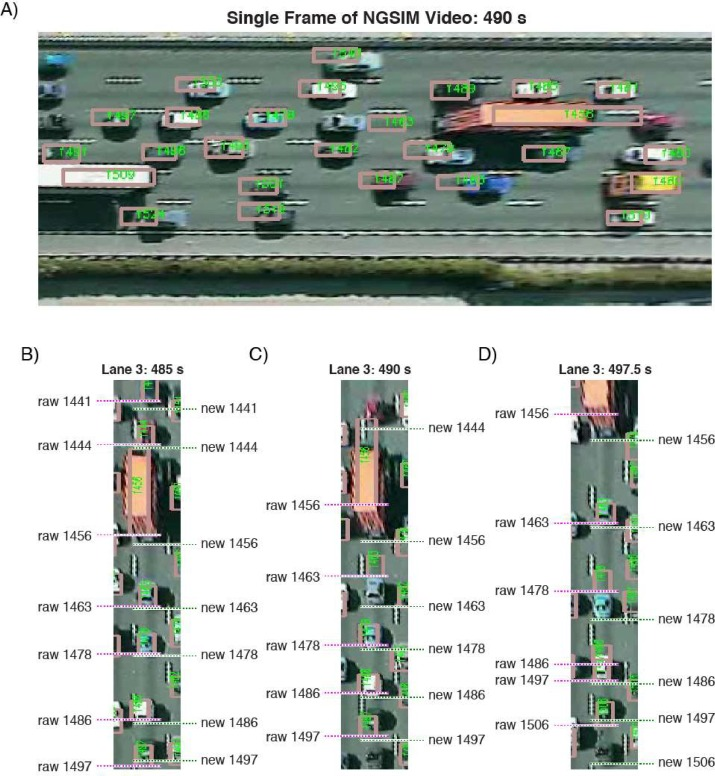
\includegraphics[width=12cm]{interpolation.jpg}
    \caption{Speed interpolation errors. (A) A typical frame from the NGSIM validation video for I-80 camera 6 at 490s. Traffic is flowing from left to right in this image. The NGSIM researchers superimposed a pink bounding box for each vehicle. A Detail of lane 3 (3rd lane from the left) from the validation video for three frames (B) 485s, (C) 490s, and (D) 497.5s. For each vehicle the rear bumper location in the NGSIM data set is shown on the left (corresponding to the upstream end of the bounding box) and is indexed by the vehicle ID, while the new rear bumper location calculated in our study is shown on the right. From Coifman et al.}
\end{figure}

The first issue is that after accounting for vehicle length, trajectories often overrun those of proceeding vehicles seemingly resulting in "collisions of trajectories". Their analysis went on to discover the second issue: that the NGSIM acceleration often exhibits unrealistically large magnitudes and likewise that the NGSIM speeds exhibit unrealistic piecewise constant behavior, which means in the dataset some vehicles maintain zero acceleration for an unrealistically long time. As shown in Fig. 3.3, %DOUBLE CHECK THE FIGURE NUMBER ONE LAST TIME
it appears as if at low speeds the NGSIM video image processing frequently linearly interpolates the trajectories between two points in space observed many seconds apart.

In order to alleviate the impact of these errors in the dataset to the model training, we dropped the particularly problematic acceleration attribute and performed sub-sectioning and time binning of the data, creating an image-like input for the model. To achieve that, the study section needed to be split into a number of sub-sections along the length of the highway. Therefore, we gave each datapoint an additional attribute, which is distance from the start of the section. The Euclidean distance was calculated simply taking the Local X and Local Y coordinates of the datapoint, since the section stretches almost straight. The section was then divided into 21 sub-sections % NEEDS EDITS
, each of which is roughly 100 feet in length. The distance attribute was then used to assign each datapoint to a sub-section, by adding the "Section ID" attribute.

\begin{figure}[ht!]
    \centering
    \includegraphics[width=15cm]{{output1.png}}
    \caption{Visualisation of vehicle speed, density, and acceleration in each road section}
\end{figure}

Then, the datapoints were aggregated using the "Section ID" attribute, and now the data at each timestamp is binned into 21 sub-sections and the average speed, density, and acceleration of the vehicles in each sub-section at each timestamp is calculated. In the beginning of the traffic observation, some parts of the study section are not filled with datapoints yet as seen in Fig. 3.4 % DOUBLE CHECK THE FIGURE NUMBER ONE LAST TIME
, so we decided to drop the first 45 seconds of the data to remove such noise in the training data. Then, time series aggregation was performed to fill as many sub-sections as possible with non-zero density and speed values at each interval, as well as further filling null values with appropriate and plausible values. For this study, zero values for density attribute and the maximum speed limit of 60 mph for speed attribute were simply used, although the average speed of vehicles in the proceeding and following grids can also be used. 

To create the 3D tensors, the Spark dataframe was converted to RDDs, and the RDDs were grouped by key and then mapped to a key-value pair, where the key is the interval ID and the value is Row objects containing the speed, density, and acceleration values of each sub-section at each interval. The key-value pairs were then converted to a numpy array in a User Defined Function, and the returned numpy arrays were stacked to create the 4D tensor, with a shape of $R^{T{\times}M{\times}N{\times}L}$, where $T$, $M$, $N$, $L$ denotes the number of timewindows (intervals), the height of grid (lanes), the width of grid (sub-sections), the number of attributes, respecitively. % include psuedo code?

Training a model to forecast the state of traffic of the future requires the past data as well as target data. Therefore, we have to provide another dimension to the tensor, creating a stack of 4D tensors of the fixed length of intervals, which results in a 5D tensor with a shape of $R^{s{\times}p{\times}M{\times}N{\times}L}$, where $s$, $p$, $M$, $N$, $L$ denotes the number of samples, the number of timewindows to look back or the prediction target timewindows, the height of grid (lanes), the width of grid (sub-sections), the number of attributes, respecitively. Furthermore, in order to provide the model an extra time for inference, the prediction target data were offset by a fixed number of intervals, which is the skip parameter. This operation was performed sliding the "window" by the time series aggregation interval, and the resulting 5D tensor was then split into training and test datasets. % include psuedo code?

\begin{figure}[ht!]
    \centering
    \includegraphics[width=14cm]{{3dto5d.png}}
    \caption{Gantt chart-like representation of the transformation of the data from 3D to 5D tensor. Firstly, 3D matrices are stacked to create a 4D tensor, and the fixed number of 4D tensors are stacked to create a stack of past data and target data. Then, they will be again stacked to create a batch, resulting in 5D tensor.}
\end{figure}

\section{Model}

The model used in this study is a Mixed Deep Learning (MDL) model, which consists of a sequence of deep learning layers which includes a Convolutional Neural Network (CNN) and a Convolutional long short term memory neural network (Conv-LSTM), which is a combination of a Convolutional Neural Network (CNN) and a Long Short-Term Memory (LSTM) network. The model was originally introduced by Lu et al.\cite{9284587} for the prediction of lane-level traffic speeds. For lane-level traffic state prediction, it is important to make the model capture the variable traffic state over time as well as behaviours of surrounding vehicles. The model is designed to effectively capture these spatial and temporal dependencies in vehicle trajectory data, and it has been shown to outperform other models such as the LSTM and the Conv-LSTM in terms of prediction accuracy. In this secftion, we first introduce the underlying ideas of MDL, which are the standard LSTM and the Conv-LSTM, then move on to the description of the Mixed Deep Learning model.

\subsection{Convolutional Long Short Term Memory Neural Network}
Conv-LSTM, which MDL is based on, is a type of neural network that combines the spatial processing capabilities of CNN with the temporal processing capabilities of an LSTM to handle spatio-temporal data. Conv-LSTM was first proposed by Shi et al \cite{NIPS2015_07563a3f}. In short, the idea is to add Convolutional operations to an LSTM cell. This section first introduces the LSTM, then extend it into Conv-LSTM.

Traditional Recurrent Neural Networks (RNNs) can track arbitary long-term dependencies in sequential data. However, while training a traditional RNN, it performs backpropagation in which it updates the weights in the network by calculating the gradient of the loss function with respect to the weights. The problem is that the longer the input sequence is, the more vulnerable it becomes to the phenomenon called vanishing gradient problem, where the gradient of the loss function becomes too small to update the weights, causing the model training to slow down or possibly come to a complete halt. % DO I NEED TO ADD MATHEMATICAL FORMULA?

In order to address this issue, Long Short-Term Memory was introduced by Hochreiter and Schmidhuber\cite{lstm}. The key idea behind LSTM is the introduction of a memory cell in the hidden layer, which is a container of the cell state $c_t$ in which information gets stored over longer periods of time. The memory cell has three special structures that allow information to selectively influence the cell state at every moment: the input gate, the forget gate, and the output gate. The input gate $i_t$ controls the input of information to the memory cell, the forget gate $f_t$ controls the removal of information from the memory cell, and the output gate $o_t$ controls what information is output from the memory cell. The gates are controlled by sigmoid activation functions $\sigma$, which output values between 0 and 1, and a tanh activation function, which outputs values between -1 and 1. The gates are trained to learn which information to keep and which information to discard.

Let $T$, $x$, $h$ be the number of the timestamps, the input vector sequences, and the output vector sequences of the hidden layer, respecitively, the structure of LSTM neural network can be written in the following equations:
\[t = 1, 2, ..., T\]
\[x = (x_{1}, x_{2},..., x_T)\]
\[h = (h_{1}, h_{2},..., h_T)\]
\[f_t = \sigma(w_{xf} x_t + w_{hf} h_{t-1} + w_{cf} \odot c_{t-1} + b_f )\]
\[i_t = \sigma(w_{xi} x_t + w_{hi} h_{t-1} + w_{ci} \odot c_{t-1} + b_i )\]
\[c_t = f_t \odot c_{t-1} + i_t \odot \tanh(w_{xc} x_t + w_{hc} h_{t-1} + b_c)\] 
\[o_t = \sigma(w_{xo} x_t + w_{ho} h_{t-1} + w_co \odot c_t + b_o)\]
\[h_t = o_t \odot \tanh(c_t)\]
where
$\odot$ denotes the Hadamard product (element-wise multiplication) of two vectors, matrices, or tensors with the same dimension;
$\sigma$ is the sigmoid activation function;
$w_{hi}$, $w_{hf}$, $w_{ho}$ and $w_{xi}$, $w_{xf}$, $w_{xo}$ are the weight matrices for the input, forget, and output gates, respectively;
$w_{ci}$, $w_{cf}$, $w_{co}$ are the weight matrices for the cell state;
$b_i$, $b_f$, $b_o$, $b_c$ are the bias terms for the input, forget, and output gates, and cell state, respectively.

\begin{figure}[ht!]
    \centering
    \includegraphics[width=14cm]{{lstmvsrnn.png}}
    \caption{The comparison between (a) RNN and (b) LSTM structures. From Lu et al.}
\end{figure}

The standard LSTM is suitable for 1D sequential data processing, and yet it is not capable of effectively capturing the contextual information of pixel data, thus it is not ideal for 2D and 3D signal processing tasks such as images and feature maps. Conv-LSTM extends the LSTM by adding convolutional operations to both the input-to-state and state-to-state transitions in the LSTM cell, which allows the model to learn spatial features as well as temporal features from the input data. The Conv-LSTM cell has the same structure as the LSTM cell, apart from the aforementioned modification to the LSTM cell. The mathmatical equations of the Conv-LSTM cell are summarised as follows according to \cite{9779153}:
\[I_t = \sigma(W_{xi} * X_t + W_{hi} * H_{t-1} + W_{ci} \odot C_{t-1} + b_i)\]
\[F_t = \sigma(W_{xf} * X_t + W_{hf} * H_{t-1} + W_{cf} \odot C_{t-1} + b_f)\]
\[C_t = F_t \odot C_{t-1} + I_t \odot \tanh(W_{xc} * X_t + W_{hc} * H_{t-1} + b_c)\]
\[O_t = \sigma(W_{xo} * X_t + W_{ho} * H_{t-1} + W_{co} \odot C_t + b_o)\]
\[H_t = O_t \odot \tanh(C_t)\]
where $*$ denotes the convolution operator. Note that $X_t$, $C_t$, $H_t$, $I_t$, $F_t$, $O_t$ $\in$ $R^{M \times N \times L}$, where $R^{M \times N \times L}$ denotes the space of the 3D tensor, and $M$, $N$, and $L$ are the height, width, and each grid feature vector of the tensor, respectively. 

\begin{figure}[ht!]
    \centering
    \includegraphics[width=14cm]{{convlstm.png}}
    \caption{Inner structure of ConvLSTM. From Shi et al.}
\end{figure}

During convolution process in the MDL model described in the following section, the widely-used filter size of 3$\times$3 was also used for this study. In order to avoid the output feature map size reduction, often resulting in the loss of information on the edges of the input feature map, the zero-padding method in which it creates zero values around the input feature map before the process was applied.

One Conv-LSTM layer can process an input tensor $X = (X_1, X_2,..., X_T)$ into an input tensor $H = (H_1, H_2,..., H_T)$, where $T$ donates the number of the timestamps. Therefore, each Conv-LSTM layer can be defined as a mapping function $F^{CL}: R^{T{\times}M{\times}N{\times}L} \rightarrow R^{T{\times}M{\times}N{\times}L^{\prime}}$, where $L$ refers to the length of one input feature vector in each grid and $L^{\prime}$ refers to the length of the output feature vector in each grid. %PARAPHRASE THIS PARAGRAPH

\subsection{Mixed Deep Learning Model}

Mixed Deep Learning (MDL) model was proposed by by Lu et al.\cite{9284587} to forecast the traffic speeds of lane sections. The structure of the MDL model is shown in Fig. 3.6. The model simplifies the study area of the road as $m{\times}n$ grids, where $m$ is the number of lanes and $n$ is the number of the road sections at one road section. Each grid represents the area of a road section and a $l{\times}w$ matrix stores values for a spatio-temporal variable such as traffic speed and vehicle density. Looking at the third to fifth dimensions of the aforementioned 5D tensor and taking each attribute (speed and vehicle density) from the aforementioned tensor, we can translate the third to fifth dimensions of the original tensor into a tensor of ${V_t}$ and ${D_t}$ with dimention of $M{\times}N{\times}1$, which contains each attribute variables during the time series aggregation interval $t$. The prediction target vector $Y_t$ contains traffic speed of all sections during the timewindow $T_h$ and length of the $Y_t$ is $T_h{\times}M{\times}N$, where $T_h$ is the forecast horizon with an offset of the "skip" parameter. % POSSIBLY MATHMATICALLY INPRECISENESS

Since it is imporant to speed up training and inference time especially when real-time inference is in mind, we attempted to downsize the model as well as reduce the number of attributes to be fed into the architecture, which differs from the original MDL model. The original MDL architecture, where the two kinds of variables (historical travel speed and vehicle density) are fed into two sperarate architectures of stacked Conv-LSTM and CNN layers, was also tested. Here, let $L_s$ and $L_q$ be the numbers of the stacked Conv-LSTM layers in the architectures for speed and vehicle density, the downsized model's $L_s$ is $1$, whereas the original model's $L_s$ and $L_q$ are $2$. Note that the downsized model has only one stream (architecture). $T_b$ represents the input historical timewindow of speed variable, and also vehicle density variable for the original MDL model. The architecture for the spatio-temporal variable for the speed attribute can be generalised and formulated as follows:
\[ (U^{L_s}_{t-T_b}, U^{L_s}_{t-T_b+1},..., U^{L_s}_{t-1}) = F^{CL}_{L_s}...F^{CL}_{l}...F^{CL}_{1} (V_{t-T_b}, V_{t-T_b+1},..., V_{t-1}) \]
\[ \hat{Y^s_{t}} = {\sigma}_r (W_s\ast{U^{L_s}_{t-1}} + b_s) \]
The original MDL model considers an additional spatio-temporal variable which is the vehicle density attribute, adding the following architecture to the model parallelly:
\[ (G^{L_q}_{t-T_b}, G^{L_q}_{t-T_b+1},...,G^{L_q}_{t-1}) = F^{CL}_{L_q}...F^{CL}_{l}...F^{CL}_{1} (D_{t-T_b}, D_{t-T_b+1},..., D_{t-1}) \]
\[ \hat{Y^q_{t}} = {\sigma}_r (W_q\ast{G^{L_q}_{t-1}} + b_q) \]
where $U^{L_s}_{t-t^{\prime}}$, $t\prime = 1, 2,..., T_b$ and $G^{L_q}_{t-t^{\prime}}$, $t\prime = 1, 2,..., T_b$ are output hidden tensors in the highest-level layers of the speed and volume, respecitively; $W_s$ and $W_q$ are the convolutional operators to further capture the spatial correlation of the high-dimensional output tensors of the Conv-LSTM layers; $b_s$ and $b_q$ are the bias tensors; $\sigma_r$ is the ReLU activation function.

Then, we flatten the output obtained from the convolutional layers $\hat{Y^{s}_t}$, followed by feeding the vector to the fully connected layer. The original architecture has an additional operation after obtaining the two outputs $\hat{Y^{s}_t}$ and $\hat{Y^q_t}$: they are flattened and fused into one vector by performing concatenation:
\[ \hat{Y_t} = W_y \times Conc[F(\hat{Y^s_t}), F(\hat{Y^q_t})] + b_y\]
where $F(\cdot)$ is the flatten operation, $Conc(\cdot)$ is the concatenation operation, $W_y$ and $b_y$ are the weight and bias, respectively. % PUT PSUDOCODE

During the training, the model is trained to minimise the mean squared error between the predicted and the actual traffic speeds using the objective function:
\[\min_{W, b} \parallel \hat{Y_t} - Y_t \parallel^2_2 + \alpha \parallel W \parallel^2_2 \]
where $\hat{Y_t}$ is the predicted speed vector and $Y_t$ is the actual speed vector; $\alpha \parallel W \parallel^2_2$ is the L2-norm regularisation term to reduce overfitting; $W$ refers to the weighted parameters in $\hat{Y_t}$; $\alpha$ is a regularisation parameter.

\begin{figure}[ht!]
    \centering
    \includegraphics[width=14cm]{{MDL.png}}
    \caption{The structure of the orginal MDL model. From Lu et al. Note that the downsized model has only one stream of speed and thus no merging operation.}
\end{figure}

\section{Real-time streaming architecture}

\begin{figure}[ht!]
    \centering
    \includegraphics[width=14cm]{{realtime_arch.png}}
    \caption{The proposed architecture of real-time prediction data pipeline.}
\end{figure}

Above this section is the description of the model training and evaluation process. In this section, we describe the architecture of the real-time prediction data pipeline. Fig. 3.9 represents the architecture. % DOUBLE CHECK THE FIGURE NUMBER ONE LAST TIME
The pipeline consists of three main components: the data ingestion component, the Kafka streaming component, and the Spark Structured Streaming component. In this study, we reprecated an API by defining a fucntion in which the 20 percent of the total datapoints reserved for testing are converted to JSON strings and ingested chunk by chunk to Kafka server every 0.1 second, which is the same as the original data collection interval. The chunk of datapoints stored in a Kafka topic are then streamed to the Spark Structured Streaming component, where the data is preprocessed and aggregated by the time series aggregation interval $t$. This operation allows Spark to further create a 3D matrix with dimension of $R^{M{\times}N{\times}L}$, which was already explained in the preprocessing section above. Note that since Spark Strcutured Streaming does not support RDD conversion, the matrix creation is performed within the Spark DataFrame API, without converting to RDDs, which is a key difference from the preprocessing process in the training section. 

After parsing the dataframe to JSON string, the data stream is again ingested to the Kafka server, but into a different Kafka topic. The data is then streamed to the Spark Structured Streaming component, where this time the dataframe is aggregated by the length of historical timewindow $T_b$. Now the dataframe contains a 4D tensor with dimension of $R^{T{\times}M{\times}N{\times}L}$ within a column. The tensor is converted to a numpy array and fed into the trained model in a User Defined Function (UDF) registered in each Spark DataFrame Row. After the UDF stores predicted speed values in a new column, the JSON string parsed from a dataframe is streamed to the Kafka server, where the predicted speed values are stored in another Kafka topic. The predicted speed values can be then visualised in real-time using a dashboard or used for various applications such as Advanced Driver-Assistance Systems (ADAS) and Autonomous Vehicles (AVs). 

\section{Kafka}
\section{Spark Structured Streaming}



\section{Evaluation method}

According to Li et al.\cite{li2024unifyinglaneleveltrafficprediction}, the lane-level traffic prediction model accuracy is evaluated typically using three key metrics: Root Mean Squared Error (RMSE), Mean Absolute Error (MAE), and Mean Absolute Percentage Error (MAPE). However, the researchers also emphasise the importance of considering the duration of its training when the model is to be used in real-time lane-level traffic prediction, where rapid response and real-time updates are essential. This paper focuses on the architecture of real-time inference, and thus instead of considering the training time, the model's inference time as well as data preprocessing time of the streaming architecture are evaluated. The formulas for the three metrics are as follows:

\[ RMSE = \sqrt{\frac{1}{n}\sum_{i=1}^{n}(\hat{Y_i} - Y_i)^2} \]
\[ MAE = \frac{1}{n}\sum_{i=1}^{n}|\hat{Y_i} - Y_i| \]
\[ MAPE = \frac{1}{n}\sum_{i=1}^{n}\frac{|\hat{Y_i} - Y_i|}{Y_i} \]
\[ Inference (Preprocessing) Time = \frac{1}{n}\sum_{i=1}^{n}t_i \]
where $\hat{Y_i}$ is the predicted speed, $Y_i$ is the actual speed during $i$-th time interval, $n$ is the total number of predicted samples, and $t_i$ is the inference / preprocessing time of the $i$th sample.

\begin{table}[ht!]
    \centering
    \begin{tabular}{ |c|c|c| }
        \hline
        Models & Input Feature & Conv-LSTM layers number\\
        \hline
        Original & speed, density & 2\\
        Original (Real Time) & speed, density & 2\\
        Downsized & speed & 1\\ 
        Downsized (Real Time) & speed & 1\\
        \hline
    \end{tabular}
\caption{List of models evaluated}
\end{table}

We compared the original MDL model and the downsized version of the model, in terms of accuracy and real-time inference time. We also compared the accuracy of non-real-time prediction with that of real-time prediction, considering the impact of datapoint losses during streaming. 

\chapter{Results}

\chapter{Discussion, Limitations and Future Work}
% Reflection on the paper with the initial objectives, etc. (refer to the student handbook)
% Mention that time series aggregation window length has to be further optimised by feature correlation analysis method
\chapter{Conclusion}

%%%%%%%%%%%%%%%%%%%%%%%%%%%%%%%%%%%%%%%%%%%%%%%%%%%%%%%%%%%%%%%%%%%%%%%%%%%%%%%%%%%%
\bibliography{refs.bib}
%\printbibliography

%%%%%%%%%%%%%%%%%%%%%%%%%%%%%%%%%%%%%%%%%%%%%%%%%%%%%%%%%%%%%%%%%%%%%%%%%%%%%%%%%%%%
\begin{appendices}

\chapter{Supplementary Materials I}

Sample text sample text sample text sample text sample text sample
text sample text sample text sample text sample text sample text
sample text sample text sample text sample text sample text.

\chapter{Supplementary Materials II}

Sample text sample text sample text sample text sample text sample
text sample text sample text sample text sample text sample text
sample text sample text sample text sample text sample text.

\end{appendices}

\end{document}
